\documentclass[14pt, aspectratio=169]{beamer}

\usepackage[T2A]{fontenc}
\usepackage[utf8]{inputenc}
\usepackage[bulgarian]{babel}
\usepackage[nointegrals]{wasysym}

\usetheme{tues}

\graphicspath{{assets/}}

\definecolor{bibnote}{HTML}{627293}

\usepackage{tikz}
\usetikzlibrary{calc, decorations.pathreplacing}

% Transistors and logic gates, drawn smaller than circuitikz draws them so that
% a whole circuit fits beside the others on one slide.
\usepackage[americanports]{circuitikz}
\ctikzset{tripoles/mos style/no arrows, bipoles/length=0.85cm}
\tikzset{
  logic title/.style={font=\footnotesize\bfseries, text=tuesnavy},
  logic block/.style={draw=tuesnavy, fill=tuesblue!12, rounded corners=2pt,
    align=center, inner sep=2pt},
}

% A step of a segmented build inside a picture, where \seg cannot be used: an
% unbraced step there leaves the pictures after it shown or hidden at the
% wrong steps. Everything in the argument is one step; nothing changes in
% other builds.
\newcommand{\segpart}[1]{%
  \ifsegmented
    \ifnum\value{beamerpauses}=1 \setcounter{beamerpauses}{2}\fi
    \uncover<+->{#1}%
  \else #1\fi}

% The toy processor of Crash Course Computer Science #7, with its English
% names, in parts so that a slide can build it up one part at a time: RAM with
% the program, the registers on the data bus, the instruction and instruction
% address registers, the control unit around them, and the ALU. Its cells are
% named - ram0 to ram7, regA to regD, iro, ira and iar - for the slides that
% draw over them.
\tikzset{
  cpu cell/.style={draw=tuesnavy, fill=white, minimum height=0.38cm,
    inner sep=1pt, font=\tiny\ttfamily},
  cpu label/.style={font=\tiny, text=gray!80!black},
  cpu step/.style={circle, inner sep=0.6pt, font=\tiny\bfseries, text=white},
}
\newcommand{\cpuram}{%
  \node[font=\scriptsize\bfseries, text=tuesnavy] at (11.95,3.1) {RAM};
  \node[cpu label] at (11.25,2.57) {address};
  \node[cpu label] at (12.325,2.57) {data};
  \foreach \addr/\data [count=\k from 0] in
      {0/0010 1110, 1/0001 1111, 2/1000 0100, 3/0100 1101, 4-12/0000 0000,
       13/0000 0000, 14/0000 0011, 15/0000 1110} {
    \node[cpu cell, minimum width=0.7cm] at (11.25,2.15-\k*0.38) {\addr};
    \node[cpu cell, minimum width=1.45cm] (ram\k) at (12.325,2.15-\k*0.38)
      {\data};
  }
  \draw[tuesnavy, thick] (10.75,2.8) rectangle (13.15,-0.85);}
\newcommand{\cpuregisters}{%
  \draw (3.35,3.3) -- (9.85,3.3) |- (10.75,2.0);
  \node[cpu label, anchor=south east] at (10.7,2.0) {data};
  \foreach \r/\x in {A/3.35, B/4.95, C/6.55, D/8.15} {
    \node[cpu cell, minimum width=1.5cm] (reg\r) at (\x,2.3)
      {\textsf{\textbf{\r}}\; 0000 0000};
    \draw (reg\r.north) -- (\x,3.3);
    \fill (\x,3.3) circle (1pt);
  }}
\newcommand{\cpuir}{%
  \node[cpu label] at (6.9,1.25) {instruction register};
  \node[cpu cell, minimum width=0.9cm] (iro) at (6.45,0.85) {0000};
  \node[cpu cell, minimum width=0.9cm] (ira) at (7.35,0.85) {0000};
  \node[cpu label] at (6.45,0.47) {opcode};
  \node[cpu cell, minimum width=1.8cm] (iar) at (6.9,-0.55) {0000 0000};
  \node[cpu label] at (6.9,-0.95) {instruction address register};
  \draw (9.5,3.3) -- (9.5,0.85) -- (ira.east);
  \fill (9.5,3.3) circle (1pt);
  \draw (ira.south) |- (8.55,0.3);
  \draw (iar.east) -| (8.55,0.3) -- (10.75,0.3);
  \node[cpu label, anchor=south east] at (10.7,0.3) {address};}
\newcommand{\cpucu}{%
  \draw[tuesnavy, thick, rounded corners=2pt] (2.6,-1.75) rectangle (8.9,1.6);
  \node[anchor=north west, font=\scriptsize\bfseries, text=tuesnavy]
    at (2.7,1.55) {control unit};
  \foreach \x in {3.35, 4.95, 6.55, 8.15} \draw (\x,2.11) -- (\x,1.6);
  \draw (8.9,-0.2) -- (10.75,-0.2);
  \node[cpu label, anchor=south east] at (10.7,-0.2) {read enable};
  \draw (8.9,-0.6) -- (10.75,-0.6);
  \node[cpu label, anchor=south east] at (10.7,-0.6) {write enable};}
\newcommand{\cpualu}{%
  \draw[fill=tuesblue!12, draw=tuesnavy] (-0.1,0.7) -- (1.7,0.7) -- (1.25,-0.9)
    -- (0.35,-0.9) -- cycle;
  \node[font=\scriptsize\bfseries, text=tuesnavy] at (0.8,-0.3) {ALU};
  \draw (2.6,1.25) -| (0.3,0.7);
  \draw (2.6,1.0) -| (1.3,0.7);
  \draw (2.6,0.1) -- (1.53,0.1) node[cpu label, midway, above] {opcode};
  \draw (1.39,-0.4) -- (2.8,-0.4);
  \foreach \f [count=\k from 0] in {O, Z, N}
    \node[cpu cell, minimum width=0.3cm] at (2.95+\k*0.3,-0.4) {\f};
  \node[cpu label] at (3.25,-0.05) {flags};
  \draw (0.8,-0.9) -- (0.8,-2.1) -| (4.2,-1.75);
  \node[cpu label, anchor=west] at (0.85,-1.55) {output};}

% The 32 bits of an IEEE 754 float, coloured by field, with a value (or
% nothing) in each cell: \floatbits{0,1,0,...}.
\colorlet{signbits}{orange!40}
\colorlet{exponentbits}{cyan!30}
\colorlet{fractionbits}{violet!20}
\newcommand{\floatbits}[1]{%
  \begin{tikzpicture}[x=0.4cm, y=0.55cm]
    \foreach \bit [count=\i from 0] in {#1} {
      \ifnum\i=0 \def\fieldcolor{signbits}%
      \else\ifnum\i<9 \def\fieldcolor{exponentbits}%
      \else\def\fieldcolor{fractionbits}\fi\fi
      \filldraw[fill=\fieldcolor, draw=white] (\i,0) rectangle ++(1,1);
      \node[font=\scriptsize\ttfamily] at (\i+0.5,0.5) {\bit};
    }
    \node[below, font=\scriptsize] at (0.5,0) {$S$};
    \node[below, font=\scriptsize] at (5,0) {експонента $E$ (8)};
    \node[below, font=\scriptsize] at (20.5,0) {дробна част $F$ (23)};
  \end{tikzpicture}%
}

\title{Преговор: представяне на данни и хардуер}
\subtitle{Операционни системи}
\author{Ангел Пенчев}
\institute{ТУЕС, XI\textsuperscript{А}}
\date{\today}

\begin{document}

\begin{frame}
  \tableofcontents
\end{frame}

\section{Организация}

\begin{frame}{Занятия}
  \begin{itemize}
    \item Два блока седмично; във всеки от тях един учебен час теория и един
      учебен час практика.
    \item За практическите занятия Ви е необходим \emph{компютър}. В случай, че
      за някой конкретен това не е така, ще предупреждавам своевременно.
  \end{itemize}
\end{frame}

\begin{frame}{Конспект - сбита версия}
  \begin{enumerate}
    \setcounter{enumi}{-1}
    \item Въведение в ОС
    \item Програмиране на \texttt{C}
    \item Памет
    \item Процесор
    \item Файлови системи
    \item Мрежи
    \item Сигурност
  \end{enumerate}
\end{frame}

\section{Преговор}

\begin{frame}{Бройни системи}
  \underline{Какво е бройна система?}
  \bigskip

  \seg
  \begin{tabular}{@{}p{0.6\textwidth}l@{}}
    $14_{(10)} = 1 \cdot 10^1 + 4 \cdot 10^0$
      & $\implies 14_{(10)}$ \\[0.3em] \seg
    $14_{(10)} = 1 \cdot 2^3 + 1 \cdot 2^2 + 1 \cdot 2^1 + 0 \cdot 2^0$
      & $\implies 1110_{(2)}$ \\[0.3em] \seg
    $14_{(10)} = 1 \cdot 3^2 + 1 \cdot 3^1 + 2 \cdot 3^0$
      & $\implies 112_{(3)}$ \\[0.3em] \seg
    $14_{(10)} = 1 \cdot 8^1 + 6 \cdot 8^0$
      & $\implies 16_{(8)}$ \\[0.3em] \seg
    $14_{(10)} = 14 \cdot 16^0$
      & $\implies 14_{(16)} \equiv E_{(16)}$
  \end{tabular}
\end{frame}

\begin{frame}{Бройни системи}
  \[
    14_{\textcolor<5>{teal}{(10)}} =
    \textcolor<3,5>{violet}{1} \cdot 2^{\textcolor<4,5>{orange}{3}} +
    \textcolor<3,5>{violet}{1} \cdot 2^{\textcolor<4,5>{orange}{2}} +
    \textcolor<3,5>{violet}{1} \cdot 2^{\textcolor<4,5>{orange}{1}} +
    \textcolor<3,5>{violet}{0} \cdot 2^{\textcolor<4,5>{orange}{0}} =
    1110_{\textcolor<2,5>{cyan}{(2)}}
  \]
  \bigskip

  \hspace*{1cm}\visible<2,5>{\textcolor{cyan}{База}}\par\smallskip
  \hspace*{1cm}\visible<3,5>{\textcolor{violet}{Коефициенти}}\par\smallskip
  \hspace*{1cm}\visible<4,5>{\textcolor{orange}{Позиции}}\par\smallskip
  \noindent\visible<5>{От значение е и \textcolor{teal}{базата} на
    първоначалната бройна система база.}
\end{frame}

\begin{frame}{Бройни системи}
  \begin{itemize}
    \item Най-важните бройни системи за нас са двоична и шестнайсетична.
    \item Първата, заради нейната тясна връзка с хардуера, върху който се
      изпълняват нашите програми. Ще бележим с префикс \texttt{0b}.
    \item Втората, защото е много лесно преобразуването ѝ към двоична и
      обратно. \emph{Защо?} Ще бележим с префикс \texttt{0x}.
  \end{itemize}
\end{frame}

\begin{frame}{Бройни системи}
  \begin{itemize}
    \item Ключовото наблюдение е, че една шестнайсетична цифра описва точно
      половин байт - т.е. четири бита. Най-голямата шестнайсетична цифра е
      \texttt{f}.
  \end{itemize}
  \seg
  \[
    \begin{aligned}
      \texttt{f}_{(16)} &= 1111_{(2)} \\
      \texttt{ff}_{(16)} &= 11111111_{(2)}
    \end{aligned}
  \]
\end{frame}

\begin{frame}{Бройни системи}
  \begin{itemize}
    \item Превръщаме от двоична към шестнайсетична, разделяйки поредицата от
      битове (започвайки от най-младшия) на групи от по четири (наричаме ги
      тетрада), и на всяка от получените групи съпоставяме съответната
      шестнайсетична цифра.
    \item Обратната посока. Превръщаме от шестнайсетична към двоична, като на
      всяка цифра съпоставяме група от по четири бита.
  \end{itemize}
\end{frame}

\begin{frame}{Десетични представки}
  Представките в системата SI умножават мерната единица по степен на 10 -
  например $1\,\text{km} = 10^3\,\text{m}$, а $1\,\text{ms} = 10^{-3}\,\text{s}$.
  \medskip

  \seg
  \noindent
  \begin{columns}[T]
    \begin{column}{0.45\textwidth}
      \centering
      \begin{tabular}{@{}lr@{}}
        \toprule
        \textbf{Представка} & \textbf{Множител} \\
        \midrule
        кило (k) & $10^{3}$ \\
        мега (M) & $10^{6}$ \\
        гига (G) & $10^{9}$ \\
        тера (T) & $10^{12}$ \\
        пета (P) & $10^{15}$ \\
        \bottomrule
      \end{tabular}
    \end{column}
    \begin{column}{0.45\textwidth}
      \seg
      \centering
      \begin{tabular}{@{}lr@{}}
        \toprule
        \textbf{Представка} & \textbf{Множител} \\
        \midrule
        мили (m) & $10^{-3}$ \\
        микро (\textmu) & $10^{-6}$ \\
        нано (n) & $10^{-9}$ \\
        пико (p) & $10^{-12}$ \\
        фемто (f) & $10^{-15}$ \\
        \bottomrule
      \end{tabular}
    \end{column}
  \end{columns}
\end{frame}

\begin{frame}{Няколко важни константи}
  \emph{Уговорка.} За нас един килобайт е 1024 байта. Аналогично имаме
  \seg
  \[
    \begin{aligned}
      1\,\text{KB} &= 1024\,\text{B} \\
      1\,\text{MB} &= 1024\,\text{KB} \\
      1\,\text{GB} &= 1024\,\text{MB} \\
      1\,\text{TB} &= 1024\,\text{GB} \\
      1\,\text{PB} &= 1024\,\text{TB}
    \end{aligned}
  \]
\end{frame}

\begin{frame}{Няколко важни константи}
  \textbf{Няма} да се придържаме към системата SI, която определя един
  килобайт като 1000 байта, а 1024 байта нарича кибибайт. Важните константи
  са:
  \seg
  \[
    \begin{aligned}
      1\,\text{KB} &= 2^{10}\,\text{B} \\
      1\,\text{MB} &= 2^{20}\,\text{B} \\
      1\,\text{GB} &= 2^{30}\,\text{B} \\
      1\,\text{TB} &= 2^{40}\,\text{B} \\
      1\,\text{PB} &= 2^{50}\,\text{B}
    \end{aligned}
  \]
\end{frame}

\begin{frame}{Няколко важни константи}
  Тяхното помнене е доста удобно, когато трябва бързо да превърнете
  произволно число - било то отместване във файл или големина на описвано
  множество от побитова карта, в размер.
\end{frame}

\begin{frame}{Индианци и яйца (Endianness)}
  \begin{itemize}
    \item \emph{Пример.} Нека имаме целочислено число, съставено от четири
      байта (\texttt{uint32\_t}). В паметта то се представя чрез поредица от
      съседни байтове - това е неговият \emph{запис}. Програмистът влага на
      тези байтове \emph{смисъл} на число, представено в двоична бройна
      система.
    \item За реда на байтовете (записа) има два общоприети варианта -
      отдясно-наляво или отляво-надясно; т.е. младшите битове се намират
      съответно или най-вдясно, или най-вляво.
  \end{itemize}
\end{frame}

\begin{frame}{Индианци и яйца (Endianness)}
  \begin{figure}
    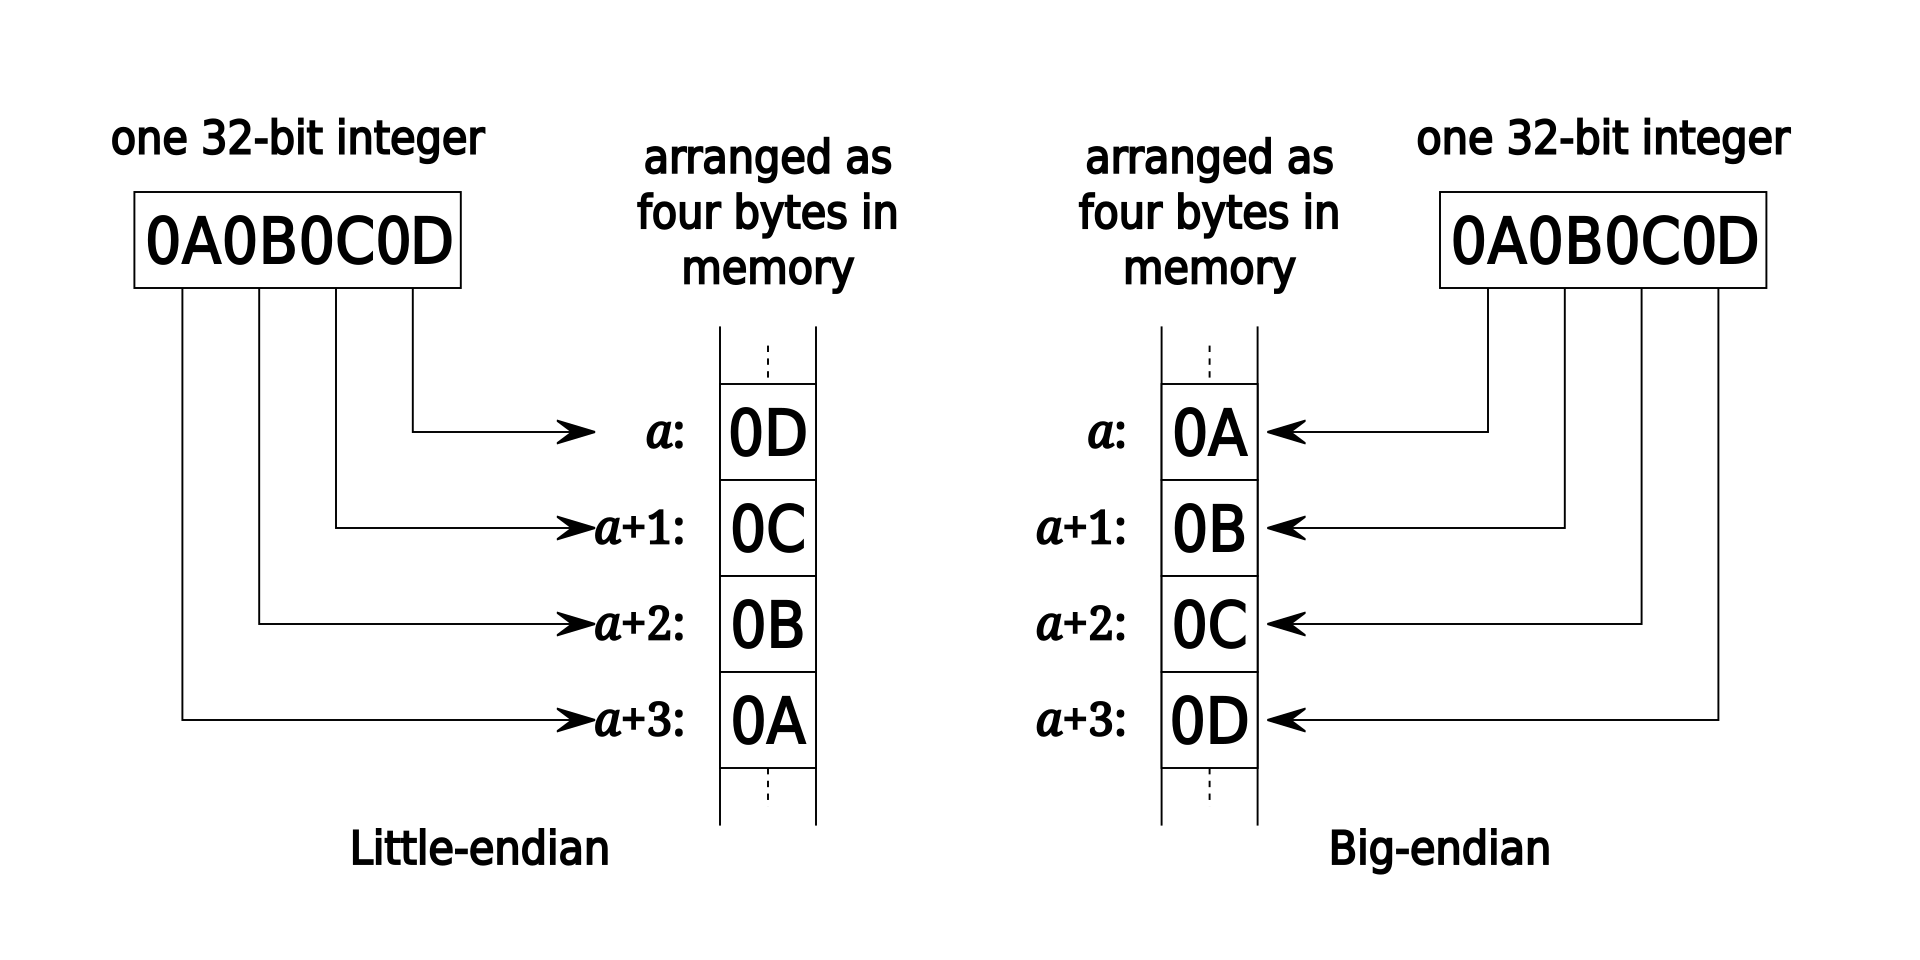
\includegraphics[height=0.55\textheight]{endianness}
    \caption{Илюстрация на endianness при 4-байтово число.}
  \end{figure}
\end{frame}

\begin{frame}{Индианци и яйца (Endianness)}
  \begin{itemize}
    \item Когато байтовете на данните са разположени отдясно-наляво, казваме,
      че се използва big endian. Обратно, ако са отляво-надясно - little
      endian.\footnote{Терминът \emph{endianness} произлиза от творбата
        „Пътешествията на Гъливер“ на Джонатан Суифт, в един епизод от която
        две групи лилипути имат спор за това от кой край трябва да се чупи
        сварено яйце - дали от малкия (little end), или от големия (big end).
        Оттам идват и съответно little-endian и big-endian. Действителна
        връзка с индианци няма. \smiley}
    \item При повечето архитектури (x86, ARM) се използва little-endian.
    \item При комуникация през мрежата се използва big-endian (още наричан
      network order).
  \end{itemize}
\end{frame}

\subsection{Упражнение 1}

\begin{frame}{Упражнение}
  \begin{itemize}
    \item Превърнете 0b111011110011 в шестнайсетична бройна система.
      \answer{0xef3}
    \item Ако горното число беше размер на файл, то колко щеше да бъде голям
      той? \answer{3KB 755B}
    \item Ако горното число беше записът в little-endian, то колко щеше да бъде
      размерът на файла? \answer{0b001111111110 = 0x3fe = 1022B}
    \item 0x8000000, 0x1000, 0x400, 0x10000. \answer{128MB, 4KB, 1KB, 64KB}
    \item Използвайте програма, написана на C, за да проверите дали машината Ви
      използва little- или big-endian за 4-байтово целочислено число.
      \emph{Подсказка.} В \texttt{gdb} използвайте команда \texttt{x/4b \&a},
      където \texttt{a} е вашата променлива.
  \end{itemize}
\end{frame}

\section{Защо двоична бройна система?}

\begin{frame}{Защо двоична бройна система?}
  \begin{itemize}
    \item Не винаги е било така. Машините на Бабидж (XIX в.), Harvard Mark I
      (1944) и ENIAC (1945) смятат в \emph{десетична} система - за всяка цифра
      има колело или брояч с 10 положения.
    \item По същото време Z3 на Конрад Цузе (1941) и ABC на Джон Атанасов и
      Клифърд Бери (1942) смятат в \emph{двоична}.\footnote{Бащата на Джон
        Атанасов, Иван Атанасов, е българин от село Бояджик.}
    \item След доклада на фон Нойман за EDVAC (1945) почти всички компютри са
      двоични. \emph{Защо?}
  \end{itemize}
\end{frame}

\begin{frame}{Защо точно две състояния?}
  \begin{columns}[c]
    \begin{column}{0.66\textwidth}
      \begin{itemize}
        \item Сигналът е напрежение - непрекъсната величина, върху която
          винаги има шум.
        \item При 2 нива всяка стойност има широк интервал и шумът трудно ги
          обърква. При 10 нива интервалите са много по-тесни.
        \item Транзисторът не е „двоичен“ - в цифровите схеми го използваме
          като ключ, напълно отворен или затворен.
      \end{itemize}
    \end{column}
    \begin{column}{0.3\textwidth}
      \centering
      \begin{tikzpicture}[x=1cm, y=0.85cm, font=\scriptsize]
        \draw[->] (-0.3,0) -- (-0.3,4.3) node[above] {$U$};
        \fill[tuesblue!25] (0,0) rectangle (1,1.4);
        \fill[gray!15] (0,1.4) rectangle (1,2.6);
        \fill[tuesblue!25] (0,2.6) rectangle (1,4);
        \node at (0.5,0.7) {\normalsize 0};
        \node at (0.5,3.3) {\normalsize 1};
        \draw (0,0) rectangle (1,4);
        \foreach \i in {0,...,9} {
          \fill[tuesblue!25] (1.6,{\i*0.4+0.06}) rectangle (2.6,{\i*0.4+0.34});
          \node[font=\tiny] at (2.1,{\i*0.4+0.2}) {\i};
        }
        \draw (1.6,0) rectangle (2.6,4);
        \node[below] at (0.5,0) {2 нива};
        \node[below] at (2.1,0) {10 нива};
      \end{tikzpicture}
    \end{column}
  \end{columns}
\end{frame}

\begin{frame}{Двоичната логика е проста}
  \begin{itemize}
    \item Две състояния са истина и лъжа - аритметиката се свежда до булева
      алгебра (Шанън, 1937), а И, ИЛИ и НЕ се изграждат от няколко транзистора.
    \item Всичко, което обработваме - числа, текст, изображения, звук,
      програми - може да се запише като поредица от битове.
    \item Не е догма. Сетун (МГУ, 1958) е троичен компютър, флаш паметите
      MLC/TLC/QLC пазят по 2-4 бита в клетка (4-16 нива на заряд), а PCIe 6.0
      предава по 2 бита наведнъж (PAM4, 4 нива). Там допълнителните грешки се
      поемат от кодове за корекция.
  \end{itemize}
\end{frame}

\begin{frame}{Цели числа без знак}
  \begin{itemize}
    \item С $N$ бита записваме $2^N$ различни стойности. Без знак (unsigned)
      това са числата от $0$ до $2^N - 1$.
  \end{itemize}
  \begin{center}
    \small
    \begin{tabular}{@{}rl@{}}
      \toprule
      \textbf{Бита} & \textbf{Обхват} \\
      \midrule
      8 & от 0 до 255 \\
      16 & от 0 до 65\,535 \\
      32 & от 0 до 4\,294\,967\,295 \\
      64 & от 0 до $\approx 1.8 \cdot 10^{19}$ \\
      \bottomrule
    \end{tabular}
  \end{center}
  \begin{itemize}
    \item Броят битове е фиксиран. Пренос, който не се побира, се губи -
      смятаме по модул $2^N$. В 8 бита $255 + 1 = 0$, като километраж на кола.
  \end{itemize}
\end{frame}

\begin{frame}{Цели числа в C}
  \begin{center}
    \small
    \begin{tabular}{@{}lrrr@{}}
      \toprule
      \textbf{Тип} & \textbf{Минимум по стандарт} & \textbf{Linux x86-64}
        & \textbf{Windows x64} \\
      \midrule
      \texttt{char} & 8 бита & 8 & 8 \\
      \texttt{short} & 16 бита & 16 & 16 \\
      \texttt{int} & 16 бита & 32 & 32 \\
      \texttt{long} & 32 бита & 64 & 32 \\
      \texttt{long long} & 64 бита & 64 & 64 \\
      \bottomrule
    \end{tabular}
  \end{center}
  \begin{itemize}
    \item Стандартът гарантира само минимални размери, реалните зависят от
      платформата - проверете със \texttt{sizeof}.
    \item Когато размерът е важен, използвайте типовете от
      \texttt{<stdint.h>}: \texttt{int8\_t}, \texttt{uint16\_t},
      \texttt{int32\_t}, \texttt{uint64\_t} и т.н.
  \end{itemize}
\end{frame}

\begin{frame}{Въпрос}
  \centering
  \vfill
  {\Large\texttt{(unsigned char)-1 == 255}}

  \bigskip
  Вярно ли е? Защо?
  \vfill
\end{frame}

\begin{frame}{Отрицателни числа - първи опит}
  \begin{itemize}
    \item Най-простата идея: най-старшият бит е знак, а останалите - големина
      (на англ. sign and magnitude).
      \[
        +5 = \texttt{0000\,0101} \qquad -5 = \texttt{1000\,0101}
      \]
    \item Два проблема:
      \begin{itemize}
        \item две нули - \texttt{0000\,0000} ($+0$) и \texttt{1000\,0000} ($-0$);
        \item обикновеното събиране вече не работи:
          $\texttt{0000\,0101} + \texttt{1000\,0101} = \texttt{1000\,1010} = -10$,
          а не $0$.
      \end{itemize}
  \end{itemize}
\end{frame}

\begin{frame}{Допълнителен код}
  \begin{itemize}
    \item В допълнителен код (на англ. two's complement) най-старшият бит
      получава \emph{отрицателно} тегло $-2^{N-1}$:
      \[
        \texttt{1111\,1011} = -128 + 64 + 32 + 16 + 8 + 2 + 1 = -5
      \]
    \item Смяна на знака: обръщаме всички битове и добавяме 1.
      \[
        5 = \texttt{0000\,0101} \;\longrightarrow\; \texttt{1111\,1010}
        \;\longrightarrow\; \texttt{1111\,1011} = -5
      \]
    \item Събирането работи без промяна, преносът се изхвърля:
      \[
        \texttt{0000\,0101} + \texttt{1111\,1011} = \texttt{(1)\,0000\,0000} = 0
      \]
  \end{itemize}
\end{frame}

\begin{frame}{Допълнителен код}
  \begin{itemize}
    \item Има само една нула, а една и съща схема събира числа със и без знак.
    \item Обхватът е от $-2^{N-1}$ до $2^{N-1} - 1$ - за 8 бита от $-128$ до
      $127$.
    \item Старшият бит все още показва знака (1 значи отрицателно), но не е
      „просто знак“ - $-1$ е \texttt{1111\,1111}, а не \texttt{1000\,0001}.
    \item Затова \texttt{(unsigned char)-1 == 255}: битовете са същите, само
      ги четем по различен начин.
  \end{itemize}
\end{frame}

% Hidden for now: it comes too early in the lecture.
\begin{frame}<0>{Цели числа в C - особености}
  \begin{itemize}
    \item От C23 стандартът изисква допълнителен код. Преди е допускал и други
      представяния, но на практика всички платформи използват него.
    \item Аритметиката без знак е по модул $2^N$, а препълване при числа със
      знак е \emph{недефинирано поведение} - компилаторът приема, че не се
      случва.
    \item Дали \texttt{char} е със знак, зависи от платформата: на x86
      обикновено е, на ARM Linux - не. Когато е важно, пишете \texttt{signed
        char} или \texttt{unsigned char}.
    \item Двоичните литерали (\texttt{0b1010}) са в стандарта от C23, а дотогава
      са разширение на GCC и Clang.
  \end{itemize}
\end{frame}

\begin{frame}{Дроби - позиции след запетаята}
  \begin{itemize}
    \item Позиционният запис продължава и надясно от запетаята - с
      отрицателни степени на основата:
      \[
        0.625_{(10)} = 6 \cdot 10^{-1} + 2 \cdot 10^{-2} + 5 \cdot 10^{-3}
      \]
    \item \emph{А в двоична?} Колко е $0.101_{(2)}$?
  \end{itemize}
\end{frame}

\begin{frame}{Дроби - позиции след запетаята}
  \begin{itemize}
    \item В двоична е същото, но степените са на 2:
      \[
        0.101_{(2)} = 1 \cdot 2^{-1} + 0 \cdot 2^{-2} + 1 \cdot 2^{-3}
          = 0.5 + 0.125 = 0.625
      \]
    \item Всяка позиция надясно е два пъти по-малка от предишната:
      \[
        2^{-1} = 0.5 \qquad 2^{-2} = 0.25 \qquad 2^{-3} = 0.125
        \qquad 2^{-4} = 0.0625
      \]
    \item Пример: $5.75 = {}$\seg $4 + 1 + 0.5 + 0.25 = 101.11_{(2)}$
  \end{itemize}
\end{frame}

\begin{frame}{Дроби - от десетична към двоична}
  \begin{itemize}
    \item Умножаваме дробната част по 2. Цялата част на резултата е следващият
      бит, а с дробната продължаваме.
    \item \emph{Защо?} Умножението по 2 мести двоичната запетая с една
      позиция надясно - първият бит след нея „излиза“ пред нея.
  \end{itemize}
  \begin{center}
    \begin{tabular}{@{}r@{${}\times 2 = {}$}l@{\qquad}c@{}}
      \toprule
      \multicolumn{2}{@{}l}{\textbf{Пресмятане}} & \textbf{Бит} \\
      \midrule
      \seg $0.625$ & $1.25$ & 1 \\
      \seg $0.25$ & $0.5$ & 0 \\
      \seg $0.5$ & $1.0$ & 1 \\
      \bottomrule
    \end{tabular}
    \qquad
    \seg
    $\implies 0.625 = 0.101_{(2)}$
  \end{center}
  \begin{itemize}
    \item Спираме, когато дробната част стане 0.
  \end{itemize}
\end{frame}

\begin{frame}{Безкрайни двоични дроби}
  \begin{columns}[c]
    \begin{column}{0.36\textwidth}
      \centering
      \small
      \begin{tabular}{@{}r@{${}\times 2 = {}$}lc@{}}
        \toprule
        \multicolumn{2}{@{}l}{\textbf{Пресмятане}} & \textbf{Бит} \\
        \midrule
        \seg $0.1$ & $0.2$ & 0 \\
        \seg $0.2$ & $0.4$ & 0 \\
        \seg $0.4$ & $0.8$ & 0 \\
        \seg $0.8$ & $1.6$ & 1 \\
        \seg $0.6$ & $1.2$ & 1 \\
        \seg $0.2$ & $0.4$ & 0 \\
        \multicolumn{3}{c}{\dots} \\
        \bottomrule
      \end{tabular}
    \end{column}
    \begin{column}{0.6\textwidth}
      \seg
      \[
        0.1 = 0.0\overline{0011}_{(2)}
      \]
      \begin{itemize}
        \item Повтаря се безкрайно - също като $\frac{1}{3} = 0.333\dots$
        \item Краен двоичен запис има само дроб със знаменател степен на 2:
          $\frac{1}{2}, \frac{3}{4}, \frac{5}{8}$ - да; $\frac{1}{10},
          \frac{1}{3}$ - не.
        \item Компютърът не може да запише 0.1 точно - пази приближение.
      \end{itemize}
    \end{column}
  \end{columns}
\end{frame}

\begin{frame}{Къде да сложим запетаята?}
  \begin{itemize}
    \item \emph{Фиксирана запетая} - например 16 бита за цялата част и 16 за
      дробната. Просто е, но обхватът е малък: от $\approx 0.000015$ до
      $\approx 65\,536$.
    \item Във физиката имат същия проблем и го решават с научен запис:
      $6.022 \cdot 10^{23}$, $1.6 \cdot 10^{-19}$. Значещите цифри и порядъкът се
      пазят поотделно.
    \item \emph{Плаваща запетая} - научен запис, но с основа 2:
      \[
        5.75 = 101.11_{(2)} = 1.0111_{(2)} \cdot 2^{2}
      \]
    \item Нормализираното число винаги започва с 1, затова тази единица не се
      записва (неявен бит).
  \end{itemize}
\end{frame}

\begin{frame}{IEEE 754 - float (32 бита)}
  \begin{center}
    \floatbits{{},{},{},{},{},{},{},{},{},{},{},{},{},{},{},{},{},{},{},{},{},{},{},{},{},{},{},{},{},{},{},{}}
  \end{center}
  \seg
  \[
    \text{стойност} = (-1)^{S} \cdot 1.F_{(2)} \cdot 2^{E - 127}
  \]
  \begin{itemize}
    \item $E$ се пази без знак. Отместването 127 позволява отрицателни степени:
      $E = 127$ означава $2^0$, $E = 1$ означава $2^{-126}$.
    \item $E = 0$ и $E = 255$ са запазени - за нулата, много малки
      (денормализирани) числа, $\pm\infty$ и NaN.
    \item \texttt{double} (64 бита): 1 + 11 + 52 бита, отместване 1023.
  \end{itemize}
\end{frame}

\begin{frame}{Пример - 5.75 като float}
  \begin{enumerate}
    \item Двоично: $5.75 = 101.11_{(2)}$
    \item Нормализираме: $1.0111_{(2)} \cdot 2^{2}$
    \item Знак: $S = 0$, защото числото е положително.
    \item Експонента: $E = 2 + 127 = 129 = \texttt{1000\,0001}_{(2)}$
    \item Дробна част: битовете след запетаята, \texttt{0111}, допълнени с нули
      до 23 бита.
  \end{enumerate}
  \seg
  \begin{center}
    \floatbits{0,1,0,0,0,0,0,0,1,0,1,1,1,0,0,0,0,0,0,0,0,0,0,0,0,0,0,0,0,0,0,0}

    \smallskip
    \seg
    $= \texttt{0x40B80000}$
  \end{center}
\end{frame}

\begin{frame}{А 0.1?}
  \begin{itemize}
    \item $0.1 = 1.1001\,1001\,1001\dots_{(2)} \cdot 2^{-4}$ - дробната част е
      безкрайна, затова след 23-тия бит закръгляме.
  \end{itemize}
  \seg
  \begin{center}
    \floatbits{0,0,1,1,1,1,0,1,1,1,0,0,1,1,0,0,1,1,0,0,1,1,0,0,1,1,0,0,1,1,0,1}

    \smallskip
    \seg
    $= \texttt{0x3DCCCCCD}$
  \end{center}
  \begin{itemize}
    \item Записаното число е $0.100000001490116119384765625$ - близо до $0.1$,
      но не $0.1$.
  \end{itemize}
\end{frame}

\begin{frame}{Въпрос}
  \centering
  \vfill
  {\Large\texttt{0.1 + 0.2 == 0.3}}

  \bigskip
  Вярно ли е?
  \vfill
\end{frame}

\begin{frame}[fragile]{0.1 + 0.2 != 0.3}
  \noindent В който и да е език за програмиране сумата в \texttt{double} е
  $0.30000000000000004$.
  \medskip

  \begin{columns}[T]
    \begin{column}{0.46\textwidth}
      \small\textbf{C}
\begin{semiverbatim}\scriptsize
double s = 0.1 + 0.2;
printf("%d\\n", s == 0.3);
// 0
\end{semiverbatim}
      \seg
      \small\textbf{JavaScript}
\begin{semiverbatim}\scriptsize
> 0.1 + 0.2 === 0.3
false
\end{semiverbatim}
    \end{column}
    \begin{column}{0.5\textwidth}
      \seg
      \small\textbf{x86-64 (NASM)}
\begin{semiverbatim}\scriptsize
a:  dq 0.1
b:  dq 0.2
c:  dq 0.3

movsd   xmm0, [a]  ; 0.1
addsd   xmm0, [b]  ; + 0.2
ucomisd xmm0, [c]  ; == 0.3?
sete    al         ; al = 0
\end{semiverbatim}
    \end{column}
  \end{columns}
  \seg
  \medskip
  \noindent\small Сумата е \texttt{0x3FD3333333333334}, а $0.3$ е
  \texttt{0x3FD3333333333333} - разликата е в последния бит.
\end{frame}

\begin{frame}{Дроби - какво следва от това}
  \begin{itemize}
    \item \texttt{float} пази около 7 значещи десетични цифри, \texttt{double} -
      около 15-16.
    \item Не сравнявайте дроби с \texttt{==}. Проверявайте дали разликата е
      достатъчно малка: \texttt{fabs(a - b) < 1e-9}.
    \item Не пазете пари във \texttt{float} - пазете цели стотинки в
      целочислен тип.
    \item Специални стойности: $1.0 / 0.0 = +\infty$, $0.0 / 0.0 =$ NaN, и NaN
      не е равно дори на себе си.
  \end{itemize}
\end{frame}

\begin{frame}{Символи - ASCII}
  \begin{itemize}
    \item Компютърът не знае какво е буква. Всеки символ е число, а таблица
      определя кое число коя буква е.
    \item ASCII (1963): 7 бита, 128 символа - латински букви, цифри,
      препинателни знаци и управляващи символи (например \texttt{'\textbackslash
        n'} е 10).
    \item В C \texttt{char} е просто малко цяло число:
      \texttt{'A' == 65 == 0b1000001}, \texttt{'a' == 97 == 0b1100001}.
    \item Таблицата е подредена нарочно: малката и главната буква се различават
      в един бит (\texttt{'a' - 'A' == 32}), а стойността на цифра получаваме с
      \texttt{c - '0'}.
  \end{itemize}
\end{frame}

\begin{frame}{Символи - кодови таблици}
  \begin{itemize}
    \item ASCII използва 7 от 8-те бита. Останалите 128 стойности всеки
      използва за своите букви - само за кирилица има CP1251, KOI8-R, ISO
      8859-5 и други.
    \item Един и същ байт е различна буква в различните таблици:
  \end{itemize}
  \seg
  \begin{center}
    \small
    \begin{tabular}{@{}lll@{}}
      \toprule
      \textbf{Байт} & \textbf{Таблица} & \textbf{Символ} \\
      \midrule
      \texttt{0xC0} & CP1251 & А \\
      \texttt{0xC0} & KOI8-R & ю \\
      \texttt{0xC0} & ISO 8859-5 & Р \\
      \bottomrule
    \end{tabular}
  \end{center}
  \begin{itemize}
    \item Текст, прочетен с грешната таблица, става безсмислица
      („кракозябри“, на англ. mojibake).
  \end{itemize}
\end{frame}

\begin{frame}{Символи - Unicode и UTF-8}
  \begin{itemize}
    \item Unicode дава на всеки символ от всички писмености уникален номер (code
      point) от U+0000 до U+10FFFF - над 1,1 милиона възможни, от които над
      150\,000 вече са заети.
    \item В началото (1991) Unicode е 16-битов, но 65\,536 символа се оказват
      малко и през 1996 г. е разширен.
    \item UTF-8 записва всеки номер с 1 до 4 байта, а ASCII символите остават
      същите единични байтове:
      \begin{center}
        \small
        \begin{tabular}{@{}lll@{}}
          A & U+0041 & \texttt{41} \\
          А (кирилско) & U+0410 & \texttt{D0 90} \\
          емоджи „усмихнато лице“ & U+1F600 & \texttt{F0 9F 98 80} \\
        \end{tabular}
      \end{center}
    \item В C \texttt{strlen("Ж") == 2} - \texttt{strlen} брои байтове, не
      символи.
  \end{itemize}
\end{frame}

\section{Компоненти на компютъра}

\begin{frame}{Компютърната система}
  \begin{center}
    \begin{tikzpicture}[
        font=\footnotesize,
        unit/.style={draw=tuesnavy, fill=tuesblue!12, rounded corners=2pt,
          align=center, minimum height=0.95cm, inner sep=3pt},
        device/.style={draw=gray!70, fill=gray!8, rounded corners=2pt,
          align=center, minimum height=0.55cm, inner sep=2pt,
          font=\scriptsize},
        link/.style={<->, >=stealth, thick, tuesnavy}]
      \node[fill=tuesblue!30, minimum width=13.6cm, minimum height=0.5cm]
        (bus) at (6.8,0) {Системна шина};
      \node[unit, minimum width=2.8cm] (cpu) at (1.5,1.5) {Процесор\\(CPU)};
      \node[unit, minimum width=2.8cm] (ram) at (1.5,-1.5)
        {Оперативна памет\\(RAM)};
      \node[unit] (disk) at (5.4,1.5) {Контролер\\на диска};
      \node[unit] (usb) at (9.3,1.5) {USB\\контролер};
      \node[unit] (video) at (12.5,1.5) {Видео\\контролер};
      \node[device] (ssd) at (5.4,3) {SSD / HDD};
      \node[device] (mouse) at (7.6,3) {мишка};
      \node[device] (keyboard) at (9.3,3) {клавиатура};
      \node[device] (printer) at (11.0,3) {принтер};
      \node[device] (monitor) at (12.5,3) {монитор};
      \foreach \n in {cpu, disk, usb, video}
        \draw[link] (\n.south) -- (\n.south |- bus.north);
      \draw[link] (ram.north) -- (ram.north |- bus.south);
      \draw[link] (ssd) -- (disk);
      \foreach \n in {mouse, keyboard, printer}
        \draw[link] (\n.south) -- (usb.north);
      \draw[link] (monitor) -- (video);
      \draw[gray, dashed, rounded corners=4pt]
        (4.1,0.55) rectangle (13.65,3.75);
      \node[anchor=north east, font=\scriptsize, text=gray!80!black]
        at (13.6,4.25) {Входно-изходни устройства};
    \end{tikzpicture}
  \end{center}
\end{frame}

\begin{frame}{Процесор и памет}
  \begin{itemize}
    \item \textbf{Процесорът (CPU)} изпълнява инструкции една след друга -
      смята, сравнява и премества данни.
    \item ОС също е програма, която процесорът изпълнява. Чрез нея той
      управлява останалите компоненти.
    \item \textbf{Оперативната памет (RAM)} пази инструкциите и данните на
      програмите, които се изпълняват в момента - и двете в една и съща памет.
    \item Всеки байт в паметта има \emph{адрес}. Такива са $a$, $a+1$, $a+2$
      от слайда за endianness.
    \item RAM е енергозависима - при изключване съдържанието ѝ се губи.
  \end{itemize}
\end{frame}

\begin{frame}{Процесорът отвътре}
  \begin{center}
    \begin{tikzpicture}[
        x=1cm, y=0.95cm, font=\footnotesize,
        unit/.style={draw=tuesnavy, fill=tuesblue!12, rounded corners=2pt,
          align=center, minimum height=0.85cm, inner sep=2pt},
        cache/.style={unit, fill=tuesblue!25},
        link/.style={<->, >=stealth, thick, tuesnavy}]
      \draw[tuesnavy, rounded corners=4pt] (0,-1.5) rectangle (11,5);
      \node[anchor=north west, font=\scriptsize\bfseries, text=tuesnavy]
        at (0.1,5) {Процесор (CPU)};
      \draw[gray, dashed, rounded corners=3pt] (0.3,0.15) rectangle (7.7,4.5);
      \node[anchor=north west, font=\scriptsize, text=gray!80!black]
        at (0.35,4.5) {Ядро};
      \node[unit, minimum width=2.8cm] (cu) at (1.95,3.35)
        {Управляващо\\устройство (CU)};
      \node[unit, minimum width=1.4cm] (alu) at (4.35,3.35) {ALU};
      \node[unit, minimum width=2cm] (reg) at (6.45,3.35) {Регистри};
      \node[cache, minimum width=2.8cm] (l1i) at (1.95,2.05)
        {L1 кеш\\за инструкции};
      \node[cache, minimum width=3cm] (l1d) at (5.95,2.05) {L1 кеш\\за данни};
      \node[cache, minimum width=6.8cm] (l2) at (4,0.8) {L2 кеш};
      \draw[gray, dashed, rounded corners=3pt] (8,0.15) rectangle (10.7,4.5);
      \node[align=center, font=\scriptsize, text=gray!80!black] at (9.35,2.3)
        {Други ядра\\със свои\\L1 и L2};
      \node[cache, minimum width=10.4cm] (l3) at (5.5,-0.75)
        {L3 кеш - общ за всички ядра};
      \node[unit, minimum width=1.6cm] (ram) at (12.6,-0.75) {RAM};
      \draw[link] (cu) -- (alu);
      \draw[link] (alu) -- (reg);
      \draw[link] (cu) -- (l1i);
      \draw[link] (reg.south) -- (reg.south |- l1d.north);
      \draw[link] (l1i.south) -- (l1i.south |- l2.north);
      \draw[link] (l1d.south) -- (l1d.south |- l2.north);
      \draw[link] (l2.south) -- (l2.south |- l3.north);
      \draw[link] (9.35,0.15) -- (9.35,0.15 |- l3.north);
      \draw[link] (l3) -- (ram);
    \end{tikzpicture}
  \end{center}
\end{frame}

\begin{frame}{Части на процесора}
  \begin{itemize}
    \item \textbf{Управляващото устройство (CU)} извлича следващата инструкция,
      декодира я и казва на останалите части какво да правят.
    \item \textbf{Аритметико-логическото устройство (ALU)} смята: събиране,
      изваждане, сравнение, AND, OR, XOR, NOT. Изградено е от логически
      елементи, а те - от транзистори.
    \item \textbf{Регистрите} са най-бързата памет - няколко десетки клетки в
      самия процесор, по 64 бита на x86-64.
    \item \textbf{Кешът} пази копие на последно използваните данни от RAM, за
      да не се чака паметта всеки път.
  \end{itemize}
\end{frame}

% Access time and size of each level as two bar charts on log scales, one row
% per level. A size is a range of typical values, so its bar is solid up to the
% smaller one and pale up to the larger. RAM is in grey, for comparison. Where
% each level sits is in the notes under the charts.
\colorlet{level-bar}{tuesblue}
\colorlet{level-pale}{tuesblue!35}
\colorlet{ram-bar}{black!50}
\colorlet{ram-pale}{black!20}
\begin{frame}{Скорост и обем по нива}
  \begin{center}
  \begin{tikzpicture}[baseline=0pt, font=\scriptsize]
    \node[anchor=south west, font=\footnotesize\bfseries, text=tuesnavy]
      at (1.6,0.3) {Време за достъп};
    \foreach \ns in {0.1, 1, 10, 100} {
      \pgfmathsetmacro\x{1.7 + (log10(\ns) + 1) * 1.0}
      \draw[black!15] (\x,0.3) -- (\x,-2.35);
      \node[below, text=black!60] at (\x,-2.35) {\ns\,ns};
    }
    \foreach \level/\ns/\lbl/\kind [count=\i from 0] in {
        Регистри/0.3/{$< 0.3$ ns}/level,
        L1/1/{$\approx 1$ ns}/level,
        L2/3/{$\approx 3$ ns}/level,
        L3/10/{$\approx 10$ ns}/level,
        RAM/100/{$\approx 100$ ns}/ram} {
      \pgfmathsetmacro\y{-\i * 0.5}
      \pgfmathsetmacro\x{1.7 + (log10(\ns) + 1) * 1.0}
      \node[anchor=east] at (1.6,\y) {\level};
      \fill[\kind-bar] (1.7,\y-0.17) rectangle (\x,\y+0.17);
      \node[anchor=west, fill=white] at (\x,\y) {\lbl};
    }
  \end{tikzpicture}%
  \hspace{0.6cm}%
  \seg
  \begin{tikzpicture}[baseline=0pt, font=\scriptsize]
    \node[anchor=south west, font=\footnotesize\bfseries, text=tuesnavy]
      at (-0.1,0.3) {Обем};
    \foreach \e/\unit in {10/KB, 20/MB, 30/GB} {
      \pgfmathsetmacro\x{(\e - 6) * 0.15}
      \draw[black!15] (\x,0.3) -- (\x,-2.35);
      \node[below, text=black!60] at (\x,-2.35) {1\,\unit};
    }
    % Sizes as powers of two: 2^15 B = 32 KB, 2^21.58 B = 3 MB, and so on.
    \foreach \lo/\hi/\lbl/\kind [count=\i from 0] in {
        7/9.5/{стотици байта}/level,
        15/16/{32-64 KB}/level,
        19/21.58/{0.5-3 MB}/level,
        23/26/{8-64 MB}/level,
        33/36/{8-64 GB}/ram} {
      \pgfmathsetmacro\y{-\i * 0.5}
      \pgfmathsetmacro\xlo{(\lo - 6) * 0.15}
      \pgfmathsetmacro\xhi{(\hi - 6) * 0.15}
      \fill[\kind-pale] (0,\y-0.17) rectangle (\xhi,\y+0.17);
      \fill[\kind-bar] (0,\y-0.17) rectangle (\xlo,\y+0.17);
      \node[anchor=west, fill=white] at (\xhi,\y) {\lbl};
    }
  \end{tikzpicture}\\
  {\scriptsize\color{black!60} Двете скали са логаритмични.}
  \end{center}
  \footnotesize
  \begin{itemize}
    \item Регистрите, L1 и L2 са във всяко ядро, L3 е общ за ядрата, а RAM е
      извън процесора.
    \item Колкото по-далеч от ALU, толкова по-голям и по-бавен. L1 е разделен
      на две - за инструкции (L1I) и за данни (L1D).
  \end{itemize}
\end{frame}

\begin{frame}[fragile]{Регистри с общо предназначение}
  \begin{itemize}
    \item Достъпни са за всяка програма - за променливи, междинни резултати
      и адреси.
    \item x86-64 има 16 такива: \texttt{rax}, \texttt{rbx}, \texttt{rcx},
      \texttt{rdx}, \texttt{rsi}, \texttt{rdi}, \texttt{rsp}, \texttt{rbp} и
      \texttt{r8}-\texttt{r15}. ARM64 има 31: \texttt{x0}-\texttt{x30}.
    \item Отделно има регистри за дроби - \texttt{xmm0} от примера с
      $0.1 + 0.2$ е такъв.
    \item Някои архитектури ги делят на регистри за данни и за адреси
      (Motorola 68000), x86-64 и ARM64 - не.
  \end{itemize}
\begin{semiverbatim}\small
    mov rax, 42      ; rax = 42
    add rax, rbx     ; rax = rax + rbx
\end{semiverbatim}
\end{frame}

\begin{frame}{Регистри за управление}
  \begin{itemize}
    \item \textbf{Програмен брояч} (PC; \texttt{rip}) - адресът на следващата
      инструкция.
    \item \textbf{Регистър на инструкцията} (IR) - текущата инструкция.
      Програмите не го виждат.
    \item \textbf{Регистър на състоянието} (PSW; \texttt{rflags} на x86-64) -
      резултатът от последното сравнение (нула, знак, пренос, препълване),
      дали прекъсванията са разрешени и режимът на
      процесора.\footnote{На x86-64 режимът е в младшите два бита на
        \texttt{cs}.}
    \item Програмата ги променя само косвено - с преходи и сравнения, а
      прекъсванията и режима - само ядрото.
  \end{itemize}
\end{frame}

% From transistor to gate. A transistor is a switch between its output and a
% constant voltage: nMOS closes on a 1 at its input, pMOS on a 0. The
% transistors come first, then which terminal is which, then how they switch.
% CMOS NOT and NAND are drawn with their transistors, each next to its gate
% symbol.
\begin{frame}{От транзистора до ALU}
  \begin{center}
  \begin{circuitikz}[baseline=(current bounding box.north), font=\scriptsize,
      terminal/.style={font=\tiny}]
    \node[logic title, anchor=west] at (-1.0,0.55) {Транзисторът е ключ};
    \node[nmos] (n) at (0,-1.05) {};
    \node[terminal, text=gray] at (-0.6,-1.5) {nMOS};
    \node[pmos, emptycircle] (p) at (0,-2.65) {};
    \node[terminal, text=gray] at (-0.6,-3.1) {pMOS};
    \segpart{
      \node[terminal, left] at (n.G) {вход};
      \draw (n.D) to[short, -o] ++(0,0.12) node[terminal, right] {изход};
      \draw (n.S) node[ground] {} node[terminal, right] {постоянно 0};
      \node[terminal, left] at (p.G) {вход};
      \draw ($(p.S)+(-0.2,0)$) -- ($(p.S)+(0.2,0)$)
        node[terminal, right] {постоянно 1};
      \draw (p.D) to[short, -o] ++(0,-0.12) node[terminal, right] {изход};}
    \segpart{
    \node at (1.95,0) {вход 0};
    \node at (2.95,0) {вход 1};
    \foreach \y/\on in {-1.05/1, -2.65/0} {
      \foreach \in/\x in {0/1.95, 1/2.95} {
        \draw (\x,\y+0.55) -- (\x,\y+0.35) (\x,\y-0.35) -- (\x,\y-0.55);
        \ifnum\in=\on
          \draw[very thick, tuesblue] (\x,\y-0.35) -- (\x,\y+0.35);
        \else
          \draw (\x,\y-0.35) -- (\x+0.25,\y+0.3);
        \fi
        \fill (\x,\y+0.35) circle (1pt) (\x,\y-0.35) circle (1pt);
      }
    }}
  \end{circuitikz}%
  \hfill\seg
  \begin{circuitikz}[baseline=(current bounding box.north), font=\scriptsize]
    \node[logic title] at (0.2,0.55) {НЕ (NOT)};
    \draw (-0.5,0) -- (0.9,0) node[right] {1};
    \draw (0,0) node[pmos, emptycircle, anchor=S] (p) {};
    \draw (p.D) -- ++(0,-0.3) coordinate (q) -- ++(0,-0.3)
      node[nmos, anchor=D] (n) {};
    \draw (n.S) node[ground] {} node[right=2pt] {0};
    \draw (q) to[short, *-o] ++(0.8,0) node[right] {Q};
    \draw (p.G) -- ++(-0.25,0) coordinate (g) -- (g |- n.G) -- (n.G);
    \draw (g |- q) to[short, *-o] ++(-0.45,0) node[left] {A};
    \draw ($(n.S)+(0.15,-1.05)$) node[not port] (gate) {};
    \draw (gate.in) -- ++(-0.2,0) node[left] {A};
    \draw (gate.out) -- ++(0.2,0) node[right] {Q};
    \node[text=gray] at ($(gate.in)+(-0.85,0)$) {=};
  \end{circuitikz}%
  \hfill\seg
  \begin{circuitikz}[baseline=(current bounding box.north), font=\scriptsize]
    \node[logic title] at (0.65,0.55) {НЕ-И (NAND)};
    \draw (-0.5,0) -- (1.8,0) node[right] {1};
    \draw (0,0) node[pmos, emptycircle, anchor=S] (pa) {};
    \draw (1.3,0) node[pmos, emptycircle, anchor=S] (pb) {};
    \draw (pa.D) -- ++(0,-0.3) coordinate (q) -| (pb.D);
    \draw (q) node[circ] {} -- ++(0,-0.3) node[nmos, anchor=D] (na) {};
    \draw (na.S) node[nmos, anchor=D] (nb) {};
    \draw (nb.S) node[ground] {} node[right=2pt] {0};
    \draw (pb.D |- q) to[short, -o] ++(0.4,0) node[right] {Q};
    \foreach \t/\in in {pa/A, pb/B, na/A, nb/B}
      \draw (\t.G) -- ++(-0.15,0) node[left] {\in};
    \draw ($(nb.S)+(2.4,0.3)$) node[nand port] (gate) {};
    \draw (gate.in 1) -- ++(-0.2,0) node[left] {A};
    \draw (gate.in 2) -- ++(-0.2,0) node[left] {B};
    \draw (gate.out) -- ++(0.2,0) node[right] {Q};
    \node[text=gray] at ($(gate.west)+(-0.85,0)$) {=};
  \end{circuitikz}
  \end{center}
  \seg
  \footnotesize
  От NAND може да се построи всеки друг елемент. AND например е NAND и NOT
  след него - 6 транзистора.
\end{frame}

% From gates to an adder: a half adder of XOR and AND, then a full adder of two
% half adders and an OR. Drawn larger than the previous slide, as there are
% fewer parts.
\begin{frame}{От транзистора до ALU}
  \begin{center}
  \begin{circuitikz}[baseline=(current bounding box.north), font=\footnotesize,
      scale=1.08, circuitikz/bipoles/length=1.0cm]
    \node[logic title, anchor=west] at (-0.3,1.0) {Полусуматор (HA)};
    \draw (2,0) node[xor port] (x) {};
    \draw (2,-1.2) node[and port] (a) {};
    \draw (x.in 1) -- ++(-1.4,0) coordinate (A) node[left] {A};
    \draw (x.in 2) -- ++(-1.4,0) coordinate (B) node[left] {B};
    \draw ($(A)+(0.35,0)$) node[circ] {} |- (a.in 1);
    \draw ($(B)+(0.7,0)$) node[circ] {} |- (a.in 2);
    \draw (x.out) -- ++(0.3,0) node[right] {S (сума)};
    \draw (a.out) -- ++(0.3,0) node[right] {C (пренос)};
    \node[anchor=north west] at (0.1,-1.85) {%
      \begin{tabular}{@{}cc|cc@{}}
        A & B & C & S \\ \hline
        0 & 0 & 0 & 0 \\
        0 & 1 & 0 & 1 \\
        1 & 0 & 0 & 1 \\
        \textcolor{tuesblue}{1} & \textcolor{tuesblue}{1}
          & \textcolor{tuesblue}{1} & \textcolor{tuesblue}{0}
      \end{tabular}};
    \node[anchor=west, text=tuesblue] at (2.6,-3.5) {$1 + 1 = 10_{(2)}$};
  \end{circuitikz}%
  \hfill\seg
  \begin{circuitikz}[baseline=(current bounding box.north), font=\footnotesize,
      scale=1.08, circuitikz/bipoles/length=1.0cm]
    \node[logic title, anchor=west] at (-0.3,1.0) {Пълен суматор (FA)};
    \node[logic block, minimum width=0.8cm, minimum height=1.0cm]
      (ha1) at (1.1,-0.9) {HA};
    \node[logic block, minimum width=0.8cm, minimum height=1.0cm]
      (ha2) at (2.7,-0.3) {HA};
    \draw (4.5,-1.65) node[or port] (o) {};
    \draw (ha1.west |- 0,-0.6) -- ++(-0.8,0) node[left] {A};
    \draw (ha1.west |- 0,-1.2) -- ++(-0.8,0) node[left] {B};
    \draw (ha2.west |- 0,0) -- ++(-2.4,0) node[left] {C\textsubscript{вх}};
    \draw (ha1.east |- 0,-0.6) -- (ha2.west |- 0,-0.6);
    \draw (ha2.east |- 0,0) -- (5.55,0) node[right] {S};
    \draw (ha2.east |- 0,-0.6) -- ++(0.35,0) |- (o.in 1);
    \draw (ha1.east |- 0,-1.2) -- ++(0.4,0) |- (o.in 2);
    \draw (o.out) -- (o.out -| 5.55,0) node[right] {C\textsubscript{изх}};
    \draw[dashed, gray, rounded corners=3pt] (0.15,0.4) rectangle (5.3,-2.45);
    \node[anchor=south east, text=gray!80!black] at (5.3,-2.45) {FA};
    \node[anchor=north west, text=gray!80!black, align=left, font=\scriptsize]
      at (0.15,-2.55)
      {Събира два бита и преноса от предишния\\разред - като събиране на ръка.};
  \end{circuitikz}
  \end{center}
\end{frame}

% From adders to the ALU. Four full adders chained by their carries add 6 + 3:
% first A, then B, then the sum a bit at a time from the right, each bit with
% the carry it passes on. The ALU computes every operation at once, and the
% operation code picks the result that comes out; the example is the code the
% control unit would send for add rax, rbx. The codes 000-100 are made up -
% every processor has its own.
\begin{frame}{От транзистора до ALU}
  \begin{center}
  \begin{circuitikz}[baseline=(current bounding box.north), font=\scriptsize,
      carry/.style={above, text=orange!90!black}]
    \node[logic title, anchor=west] at (-0.95,1.5) {4-битов суматор};
    \foreach \k in {0,...,3} {
      \pgfmathsetmacro\x{\k * 1.5}
      \node[logic block, minimum width=0.9cm, minimum height=0.8cm]
        at (\x,0) {FA};
      \draw (\x-0.2,0.4) -- ++(0,0.35) (\x+0.2,0.4) -- ++(0,0.35)
        (\x,-0.4) -- ++(0,-0.35);
      \draw[<-, >=stealth] (\x+0.45,0) -- (\x+1.05,0);
    }
    \draw[->, >=stealth] (-0.45,0) -- (-0.95,0);
    \node[carry] at (5.25,0) {0};
    \segpart{
      \foreach \a [count=\k from 0] in {0,1,1,0}
        \node[above, text=tuesblue] at (\k*1.5-0.2,0.75) {\a};
      \node[anchor=west, text=tuesblue] at (-0.95,-1.45) {A = 0110 = 6};}
    \segpart{
      \foreach \b [count=\k from 0] in {0,0,1,1}
        \node[above, text=violet] at (\k*1.5+0.2,0.75) {\b};
      \node[anchor=west, text=violet] at (-0.95,-1.85) {B = 0011 = 3};}
    \segpart{
      \node[below] at (4.5,-0.75) {1};
      \node[carry] at (3.75,0) {0};
      \node[anchor=north west, text=orange!90!black, align=left]
        at (2.0,-1.2) {преносът върви\\отдясно наляво};}
    \segpart{
      \node[below] at (3.0,-0.75) {0};
      \node[carry] at (2.25,0) {1};}
    \segpart{
      \node[below] at (1.5,-0.75) {0};
      \node[carry] at (0.75,0) {1};}
    \segpart{
      \node[below] at (0,-0.75) {1};
      \node[carry] at (-0.7,0) {0};
      \node[anchor=west] at (-0.95,-2.25) {S = 1001 = 9};
      \node[anchor=north west, text=gray!80!black, align=left, font=\tiny]
        at (-0.95,-2.6)
        {Изваждане: $A - B = A + \overline{B} + 1$ - същият\\
         суматор, с обърнати битове на B и входен пренос 1.};}
  \end{circuitikz}%
  \hfill\seg
  \begin{circuitikz}[baseline=(current bounding box.north), font=\scriptsize,
      op/.style={logic block, minimum width=1.25cm, minimum height=0.36cm,
        inner sep=1pt, font=\tiny}]
    \node[logic title, anchor=west] at (-0.4,1.5) {ALU};
    \node[left] at (0,1.15) {A, B};
    \draw[very thick] (0,1.15) -- (0,-2.15);
    \foreach \op/\code [count=\k from 0] in
        {A + B/000, A $-$ B/001, A AND B/010, A OR B/011, A XOR B/100,
         \dots/{}} {
      \pgfmathsetmacro\y{0.6 - \k * 0.5}
      \draw[thick] (0,\y) -- (0.25,\y);
      \node[op] at (0.88,\y) {\op};
      \draw (1.5,\y) -- (2.1,\y)
        node[midway, above=-1pt, font=\tiny, text=gray!80!black] {\code};
    }
    \draw[fill=tuesblue!25, draw=tuesnavy] (2.1,0.8) -- (2.55,0.45)
      -- (2.55,-1.95) -- (2.1,-2.3) -- cycle;
    \node[rotate=90, font=\tiny] at (2.33,-0.75) {избор};
    \node[logic block, minimum width=0.8cm, minimum height=0.5cm] (cu)
      at (2.33,-2.95) {CU};
    \draw (2.33,-2.13) -- (cu.north)
      node[midway, right, font=\tiny] {код на операцията};
    \draw[->, >=stealth, very thick] (2.55,-0.75) -- (3.8,-0.75)
      node[right] {резултат};
    \draw[->, >=stealth] (3.1,-0.75) |- (3.5,-1.6)
      node[right, align=left] {флагове\\(rflags)};
    \fill (3.1,-0.75) circle (1.5pt);
    \segpart{
      \node[op, fill=tuesblue!45, very thick] at (0.88,0.6) {A + B};
      \draw[very thick, tuesblue] (1.5,0.6) -- (2.1,0.6);
      \node[left, text=tuesblue, font=\tiny] at (2.33,-2.4) {000};
      \node[anchor=east, align=right] (instr) at (1.6,-2.95)
        {\texttt{add rax, rbx}\\{\color{gray!80!black}\texttt{48 01 D8}}};
      \draw[->, >=stealth] (instr.east) -- (cu.west);}
  \end{circuitikz}
  \end{center}
\end{frame}

\begin{frame}{Памет и устройства за съхранение}
  \begin{center}
    \small
    \begin{tabular}{@{}llll@{}}
      \toprule
      & \textbf{Пази данните без ток} & \textbf{Типичен обем}
        & \textbf{Време за достъп} \\
      \midrule
      \seg RAM & не & 8-64 GB & $\approx 100$ ns \\
      \seg SSD & да & 0.25-4 TB & $\approx 0.1$ ms \\
      \seg HDD & да & 1-30 TB & $\approx 10$ ms \\
      \bottomrule
    \end{tabular}
  \end{center}
  \begin{itemize}
    \item Дисковете са енергонезависими и много по-обемни, но SSD е около
      1000 пъти по-бавен от RAM, а HDD - около 100\,000 пъти.
    \item Ако достъпът до RAM траеше 1 секунда, четене от SSD би отнело около
      17 минути, а от HDD - повече от ден.
  \end{itemize}
\end{frame}

% Memory, after Crash Course Computer Science #6, with its English names. A
% gate whose output feeds back into its input keeps its value: the AND-OR
% latch. Two more AND gates in front of it make a gated latch, which takes the
% value of data in only while write enable is on.
\begin{frame}{От логическия елемент до RAM}
  \begin{center}
  \begin{circuitikz}[baseline=(current bounding box.north), font=\scriptsize]
    \node[logic title, anchor=west] at (-0.9,1.2) {AND-OR latch};
    \draw (1.4,0) node[or port] (or) {};
    \draw (2.9,-0.45) node[and port] (and) {};
    \draw (1.4,-1.1) node[not port] (not) {};
    \draw (or.out) -| ($(and.in 1)+(-0.3,0)$) -- (and.in 1);
    \draw (not.out) -| ($(and.in 2)+(-0.15,0)$) -- (and.in 2);
    \draw (and.out) -- ++(0.9,0) node[right] {Q};
    \draw ($(and.out)+(0.45,0)$) node[circ] {} |- (0.5,0.7) |- (or.in 1);
    \draw (or.in 2) -- ++(-0.8,0) node[left] {set};
    \draw (not.in) -- ++(-0.5,0) node[left] {reset};
    \node[anchor=north west] at (-0.6,-1.6) {%
      \begin{tabular}{@{}cc|c@{\quad}l@{}}
        set & reset & Q & \\ \hline
        1 & 0 & 1 & \color{gray!80!black} записва 1 \\
        0 & 1 & 0 & \color{gray!80!black} записва 0 \\
        0 & 0 & Q & \color{tuesblue} помни
      \end{tabular}};
  \end{circuitikz}%
  \hfill\seg
  \begin{circuitikz}[baseline=(current bounding box.north), font=\scriptsize]
    \node[logic title, anchor=west] at (-1.9,1.2) {Gated latch};
    \draw (2.0,0) node[and port] (a1) {};
    \draw (2.0,-1.2) node[and port] (a2) {};
    \draw (a2.in 2) -- ++(-0.35,0) node[not port, anchor=out] (nd) {};
    \draw (a1.in 1) -- ++(-1.9,0) coordinate (d) node[left] {data in};
    \draw ($(d)+(0.3,0)$) node[circ] {} |- (nd.in);
    \draw (a1.in 2) -- ++(-0.2,0) coordinate (we) -- (we |- a2.in 1)
      -- (a2.in 1);
    \draw (d |- 0,-0.6) node[left] {write enable} -- (we |- 0,-0.6)
      node[circ] {};
    \node[logic block, minimum width=1.0cm, minimum height=1.75cm,
      font=\tiny] (latch) at (3.45,-0.6) {AND-OR\\latch};
    \draw (a1.out) -- (a1.out -| latch.west) node[right, font=\tiny] {set};
    \draw (a2.out) -- (a2.out -| latch.west) node[right, font=\tiny] {reset};
    \draw (latch.east) -- ++(0.45,0) node[right] {data out};
    \draw[dashed, gray, rounded corners=3pt] (-0.15,0.45) rectangle (4.2,-1.95);
    \node[anchor=south east, text=gray!80!black] at (4.2,-1.95) {gated latch};
    \node[anchor=north west, align=left, text=gray!80!black] at (-0.15,-2.1)
      {write enable = 0: изходът не се променя\\
       write enable = 1: data out = data in};
  \end{circuitikz}
  \end{center}
  \seg
  \footnotesize
  Изходът се връща обратно във входа на OR - затова схемата помни един бит,
  докато има ток.
\end{frame}

% Latches in a row are a register; in a grid they are memory. The latch at a
% row and a column is chosen when both its lines are on, so 256 latches need
% 16 row lines, 16 column lines and three shared ones - data, write enable and
% read enable - instead of an input and an output for each and a write enable.
% The address 1100 1000 selects row 12, column 8.
\begin{frame}{От логическия елемент до RAM}
  \begin{center}
  \begin{circuitikz}[baseline=(current bounding box.north), font=\scriptsize]
    \node[logic title, anchor=west] at (-1.4,1.2) {8-битов регистър};
    \draw (-0.5,0) node[left, align=right] {write\\enable} -- (3.85,0);
    \foreach \bit [count=\k from 0] in {0,1,0,0,0,0,0,1} {
      \pgfmathsetmacro\x{\k * 0.55}
      \node[logic block, minimum width=0.4cm, minimum height=0.6cm]
        at (\x,0) {};
      \draw (\x,0.3) -- ++(0,0.3) node[above, text=tuesblue] {\bit};
      \draw (\x,-0.3) -- ++(0,-0.3) node[below] {\bit};
    }
    \node[left] at (-0.25,0.75) {data in};
    \node[left] at (-0.25,-0.75) {data out};
    \node[anchor=north west, text=gray!80!black, align=left] at (-1.4,-1.3)
      {Всеки latch пази един бит,\\
       а write enable е общ за всички.\\[0.4em]
       Регистрите на x86-64 са по 64 бита.};
  \end{circuitikz}%
  \hfill\seg
  \begin{circuitikz}[baseline=(current bounding box.north), font=\scriptsize]
    \node[logic title, anchor=west] at (-1.2,1.2) {Матрица 16 × 16 = 256 бита};
    \foreach \i in {0,...,15}
      \foreach \j in {0,...,15}
        \fill[tuesblue!15] (\j*0.17,-\i*0.17) rectangle ++(0.13,-0.13);
    \foreach \j in {0,...,15}
      \fill[tuesblue!40] (\j*0.17,-12*0.17) rectangle ++(0.13,-0.13);
    \foreach \i in {0,...,15}
      \fill[tuesblue!40] (8*0.17,-\i*0.17) rectangle ++(0.13,-0.13);
    \fill[tuesnavy] (8*0.17,-12*0.17) rectangle ++(0.13,-0.13);
    \node[logic block, minimum width=0.3cm, minimum height=2.7cm,
      inner sep=0pt] (rows) at (-0.3,-1.34) {};
    \node[rotate=90, font=\tiny] at (rows) {ред};
    \node[logic block, minimum width=2.7cm, minimum height=0.3cm,
      inner sep=0pt] (cols) at (1.34,0.3) {};
    \node[font=\tiny] at (cols) {колона};
    \draw (rows.west |- 0,-1.34) -- ++(-0.15,0) node[left, text=tuesblue]
      {\texttt{1100}};
    \draw (cols.north) -- ++(0,0.2) node[above, text=tuesblue]
      {\texttt{1000}};
    \draw[gray] (1.5,-2.04) -- (3.0,-0.45);
    \draw[gray] (1.5,-2.17) -- (3.0,-2.35);
    \draw[gray, rounded corners=3pt] (3.0,-0.3) rectangle (6.2,-2.5);
    \draw (4.4,-1.75) node[and port] (sel) {};
    \draw (sel.in 1) -- ++(-0.2,0) node[left, font=\tiny] {ред};
    \draw (sel.in 2) -- ++(-0.2,0) node[left, font=\tiny] {колона};
    \node[logic block, minimum width=0.8cm, minimum height=0.55cm,
      font=\tiny] (cell) at (5.35,-1.75) {latch};
    \draw (sel.out) -- (cell.west);
    \draw (cell.north) -- ++(0,0.2) node[above, font=\tiny, text=gray!80!black,
      align=center, inner sep=1pt] {data,\\write enable,\\read enable};
    \node[anchor=north west, align=left] at (-1.2,-2.85)
      {Адрес \texttt{1100 1000}: ред 12, колона 8.\\
       {\color{gray!80!black} 16 + 16 + 3 = 35 проводника}\\
       {\color{gray!80!black} вместо 2 $\cdot$ 256 + 1 = 513}};
  \end{circuitikz}
  \end{center}
\end{frame}

% Eight 256-bit matrices behind one address store a byte at each of 256
% addresses - here 01000001, the letter A. Real RAM is built the same way, but
% its cell is a transistor and a capacitor rather than a latch: denser, though
% it forgets unless refreshed. Latch-like SRAM cells are kept for the caches.
\begin{frame}{От логическия елемент до RAM}
  \begin{center}
  \begin{circuitikz}[baseline=(current bounding box.north), font=\scriptsize]
    \node[logic title, anchor=west] at (-1.1,1.2) {256 байта};
    \draw[very thick] (-0.6,0.75) node[left] {адрес} -- (4.85,0.75);
    \foreach \bit [count=\k from 0] in {0,1,0,0,0,0,0,1} {
      \pgfmathsetmacro\x{\k * 0.65}
      \draw (\x,0.75) -- (\x,0.45);
      \fill (\x,0.75) circle (1.2pt);
      \foreach \i in {0,...,3}
        \foreach \j in {0,...,3}
          \fill[tuesblue!30] (\x-0.27+\j*0.14,0.43-\i*0.14)
            rectangle ++(0.11,-0.11);
      \draw (\x,-0.15) -- ++(0,-0.3) node[below] {\bit};
    }
    \draw[decorate, decoration={brace, mirror, amplitude=4pt}]
      (-0.3,-0.95) -- (4.85,-0.95)
      node[midway, below=5pt] {1 байт: \texttt{01000001} = A};
    \node[anchor=north west, align=left] at (-1.1,-1.75)
      {8 матрици с общ 8-битов адрес:\\
       256 адреса $\times$ 1 байт = 256 байта.\\[0.4em]
       {\color{gray!80!black} С 32-битов адрес - $2^{32}$ B = 4 GB.}};
  \end{circuitikz}%
  \hfill\seg
  \begin{circuitikz}[baseline=(current bounding box.north), font=\scriptsize]
    \node[logic title, anchor=west] at (-0.4,1.2) {Клетката в паметта};
    \node[font=\footnotesize\bfseries] at (0.75,0.75) {SRAM};
    \draw (0.75,0.1) node[not port] (i1) {};
    \draw (0.75,-0.7) node[not port, xscale=-1] (i2) {};
    \draw (i1.out) -- ++(0.2,0) |- (i2.in);
    \draw (i2.out) -- ++(-0.2,0) |- (i1.in);
    \node[anchor=north, align=center] at (0.75,-1.6)
      {latch от 6\\транзистора\\[0.3em]
       {\color{gray!80!black} бърза,}\\{\color{gray!80!black} но голяма}\\
       {\color{tuesblue} кеш}};
    \node[font=\footnotesize\bfseries] at (3.8,0.75) {DRAM};
    \draw (2.95,0.55) node[left, font=\tiny] {колона} -- (2.95,-1.35);
    \node[nmos] (t) at (3.7,-0.1) {};
    \draw (t.D) |- (2.95,0.45) node[circ] {};
    \draw (t.G) -- (2.6,0 |- t.G) node[left, font=\tiny] {ред};
    \draw (t.S) to[C] ++(0,-0.6) node[ground] {};
    \node[anchor=north, align=center] at (3.7,-1.6)
      {1 транзистор и\\1 кондензатор\\[0.3em]
       {\color{gray!80!black} плътна, но}\\{\color{gray!80!black} се опреснява}\\
       {\color{tuesblue} RAM}};
  \end{circuitikz}
  \end{center}
  \seg
  \footnotesize
  Random access: всеки адрес се чете и записва еднакво бързо, в произволен ред.
\end{frame}

% The processor of the first practice, after Crash Course Computer Science
% #7: RAM with the program, four registers on the data bus, the instruction
% register and the instruction address register inside the control unit, and
% the ALU. It is built up a part at a time, as in the video.
\begin{frame}{От ALU и RAM до процесора}
  \begin{center}
  \begin{tikzpicture}
    \cpuram
    \segpart{\cpuregisters}
    \segpart{\cpuir}
    \segpart{\cpucu}
    \segpart{\cpualu}
  \end{tikzpicture}
  \end{center}
\end{frame}

% The four instructions of the toy processor, and the program in its RAM
% decoded a line at a time: opcode in blue, operand in orange. What each line
% does is on the next slides.
\begin{frame}{От ALU и RAM до процесора}
  \begin{center}
  \begin{tikzpicture}[baseline=(current bounding box.north), font=\scriptsize]
    \node[logic title, anchor=west] at (-0.1,0.5) {Инструкции};
    \node[anchor=north west] at (-0.1,0.2) {%
      \begin{tabular}{@{}l@{\hspace{0.6em}}l@{\hspace{0.6em}}l@{\hspace{0.6em}}l@{}}
        \toprule
        instruction & opcode & operand & действие \\
        \midrule
        \texttt{LOAD\_A} & \texttt{0010} & адрес & A = RAM[адрес] \\
        \texttt{LOAD\_B} & \texttt{0001} & адрес & B = RAM[адрес] \\
        \texttt{STORE\_A} & \texttt{0100} & адрес & RAM[адрес] = A \\
        \texttt{ADD} & \texttt{1000} & регистри & втори = първи + втори \\
        \bottomrule
      \end{tabular}};
    \node[anchor=north west, text=gray!80!black] at (-0.1,-2.3)
      {Регистри: A = \texttt{00}, B = \texttt{01}, C = \texttt{10},
       D = \texttt{11}};
  \end{tikzpicture}%
  \hfill\seg
  \begin{tikzpicture}[baseline=(current bounding box.north), font=\scriptsize]
    \node[logic title, anchor=west] at (-0.2,0.5) {Програмата в RAM};
    \node[cpu label, anchor=east] at (0.3,0.05) {address};
    \foreach \x/\h in {0.5/data, 2.05/instruction}
      \node[cpu label, anchor=west] at (\x,0.05) {\h};
    \draw[gray] (-0.45,-0.15) -- (4.0,-0.15);
    \foreach \addr/\op/\arg/\ins [count=\k from 1] in
        {0/0010/1110/LOAD\_A 14, 1/0001/1111/LOAD\_B 15, 2/1000/0100/ADD B{,} A,
         3/0100/1101/STORE\_A 13} {
      \segpart{
        \node[anchor=east] at (0.3,-\k*0.45) {\addr};
        \node[anchor=west, font=\scriptsize\ttfamily] at (0.5,-\k*0.45)
          {\textcolor{tuesblue}{\op}\,\textcolor{orange!90!black}{\arg}};
        \node[anchor=west, font=\scriptsize\ttfamily] at (2.05,-\k*0.45)
          {\ins};}
    }
    \segpart{
      \foreach \addr/\data/\val [count=\k from 6] in
          {14/0000 0011/3, 15/0000 1110/14} {
        \node[anchor=east] at (0.3,-\k*0.45) {\addr};
        \node[anchor=west, font=\scriptsize\ttfamily] at (0.5,-\k*0.45)
          {\data};
        \node[anchor=west, text=gray!80!black] at (2.05,-\k*0.45)
          {данни: \val};
      }
      \node[anchor=west, text=gray!80!black] at (-0.2,-5*0.45) {\dots};}
  \end{tikzpicture}
  \end{center}
\end{frame}

% One turn of the control unit, for the instruction at address 0: fetch it
% into the instruction register, decode its opcode, execute it - here, read
% address 14 into register A - and move to the next address.
\begin{frame}{Изпълнение на програмата}
  \begin{center}
  \begin{tikzpicture}[legend/.style={anchor=west, font=\tiny}]
    \cpuram \cpuregisters \cpuir \cpucu \cpualu
    \segpart{
      \draw[very thick, tuesblue] (iar.east) -| (8.55,0.3) -- (10.75,0.3);
      \node[cpu cell, minimum width=1.45cm, fill=tuesblue!25] at (ram0)
        {0010 1110};
      \draw[very thick, tuesblue] (10.75,2.0) -- (9.85,2.0) -- (9.85,3.3)
        -- (9.5,3.3) -- (9.5,0.85) -- (ira.east);
      \node[cpu cell, minimum width=0.9cm, fill=tuesblue!25] at (iro) {0010};
      \node[cpu cell, minimum width=0.9cm, fill=tuesblue!25] at (ira) {1110};
      \node[cpu step, fill=tuesblue] at (9.5,1.9) {1};
      \node[legend] at (9.2,-1.15) {\textcolor{tuesblue}{\textbf{1 fetch:}}
        IR = RAM[IAR] = \texttt{0010 1110}};}
    \segpart{
      \draw[->, >=stealth, thick, tuesnavy] (iro.west) -- ++(-0.45,0)
        node[left, font=\tiny\ttfamily] (decoded) {LOAD\_A};
      \node[cpu step, fill=tuesnavy, left] at (decoded.west) {2};
      \node[legend] at (9.2,-1.45) {\textcolor{tuesnavy}{\textbf{2 decode:}}
        \texttt{0010} = \texttt{LOAD\_A}};}
    \segpart{
      \draw[very thick, orange] (ira.south) |- (8.55,0.3) -- (10.75,0.3);
      \node[cpu cell, minimum width=1.45cm, fill=orange!30] at (ram6)
        {0000 0011};
      \draw[very thick, orange] (8.9,-0.2) -- (10.75,-0.2);
      \draw[very thick, orange] (10.75,2.0) -- (9.85,2.0) -- (9.85,3.3)
        -- (3.35,3.3) -- (regA.north);
      \node[cpu cell, minimum width=1.5cm, fill=orange!30] at (regA)
        {\textsf{\textbf{A}}\; 0000 0011};
      \node[cpu step, fill=orange] at (5.75,3.3) {3};
      \node[legend] at (9.2,-1.75) {\textcolor{orange!90!black}{\textbf{3
        execute:}} A = RAM[\texttt{1110}] = \texttt{0000 0011}};}
    \segpart{
      \node[cpu cell, minimum width=1.8cm, fill=gray!20] at (iar) {0000 0001};
      \node[cpu step, fill=gray] at (5.75,-0.55) {4};
      \node[legend] at (9.2,-2.05) {\textcolor{gray}{\textbf{4}} IAR = IAR + 1,
        и отначало};}
  \end{tikzpicture}
  \end{center}
\end{frame}

% The whole program, an instruction at a time: what the instruction address
% register pointed at, what was fetched, and the registers and address 13 after
% it ran. What changed is in blue.
\begin{frame}{Изпълнение на програмата}
  \begin{center}
  \begin{tikzpicture}[font=\scriptsize, val/.style={font=\scriptsize\ttfamily},
      new/.style={val, text=tuesblue}]
    \foreach \x/\h in {0.65/IAR, 2.35/IR, 4.0/instruction, 5.85/A, 7.7/B,
        9.55/RAM[13]}
      \node[cpu label] at (\x,0) {\h};
    \draw[gray] (-0.2,-0.2) -- (10.5,-0.2);
    \node[val] at (0.65,-0.5) {0000 0000};
    \node[text=gray!80!black] at (4.0,-0.5) {начало};
    \foreach \x in {5.85, 7.7, 9.55} \node[val] at (\x,-0.5) {0000 0000};
    \segpart{
      \node[val] at (0.65,-0.95) {0000 0000};
      \node[val] at (2.35,-0.95) {0010 1110};
      \node[val] at (4.0,-0.95) {LOAD\_A 14};
      \node[new] at (5.85,-0.95) {0000 0011};
      \node[val] at (7.7,-0.95) {0000 0000};
      \node[val] at (9.55,-0.95) {0000 0000};}
    \segpart{
      \node[val] at (0.65,-1.4) {0000 0001};
      \node[val] at (2.35,-1.4) {0001 1111};
      \node[val] at (4.0,-1.4) {LOAD\_B 15};
      \node[val] at (5.85,-1.4) {0000 0011};
      \node[new] at (7.7,-1.4) {0000 1110};
      \node[val] at (9.55,-1.4) {0000 0000};}
    \segpart{
      \node[val] at (0.65,-1.85) {0000 0010};
      \node[val] at (2.35,-1.85) {1000 0100};
      \node[val] at (4.0,-1.85) {ADD B, A};
      \node[new] at (5.85,-1.85) {0001 0001};
      \node[val] at (7.7,-1.85) {0000 1110};
      \node[val] at (9.55,-1.85) {0000 0000};
      \node[anchor=north west, align=left, text=gray!80!black] at (-0.2,-3.0)
        {\texttt{ADD}: CU подава B и A на ALU с opcode за събиране. Изходът,
         3 + 14 = 17,\\отива в A, а флаговете O, Z и N са 0.};}
    \segpart{
      \node[val] at (0.65,-2.3) {0000 0011};
      \node[val] at (2.35,-2.3) {0100 1101};
      \node[val] at (4.0,-2.3) {STORE\_A 13};
      \node[val] at (5.85,-2.3) {0001 0001};
      \node[val] at (7.7,-2.3) {0000 1110};
      \node[new] at (9.55,-2.3) {0001 0001};}
    \segpart{
      \node[val] at (0.65,-2.75) {0000 0100};
      \node[val] at (2.35,-2.75) {0000 0000};
      \node[text=orange!90!black] at (4.0,-2.75) {?};
      \node[anchor=west, text=orange!90!black] at (4.95,-2.75)
        {няма такава инструкция};
      \node[anchor=north west, align=left] at (-0.2,-3.75)
        {Програмата свършва на адрес 3, но процесорът не знае това -\\
         продължава с каквото има на адрес 4.};}
  \end{tikzpicture}
  \end{center}
\end{frame}

% The same program in NASM for x86-64, from the first practice: register A is
% rax, B is rbx, and addresses 13, 14 and 15 are the labels result, x and y.
% The machine code is what objdump -d -M intel shows for it. Unlike the toy
% processor, a real program has to ask the kernel to end it.
\begin{frame}{Същата програма на x86-64}
  \begin{center}
  \begin{tikzpicture}[font=\scriptsize, code/.style={font=\scriptsize\ttfamily}]
    \node[logic title, anchor=west] at (-0.1,0.5) {Схемата};
    \node[logic title, anchor=west] at (3.4,0.5) {NASM};
    \node[logic title, anchor=west] at (7.6,0.5) {Машинен код};
    \foreach \toy [count=\k from 0] in
        {LOAD\_A 14, LOAD\_B 15, ADD B{,} A, STORE\_A 13}
      \node[code, anchor=west] at (-0.1,-\k*0.45) {\toy};
    \segpart{
      \foreach \asm [count=\k from 0] in
          {mov rax{,} [x], mov rbx{,} [y], add rax{,} rbx,
           mov [result]{,} rax} {
        \draw[->, >=stealth, gray] (2.0,-\k*0.45) -- (3.2,-\k*0.45);
        \node[code, anchor=west] at (3.4,-\k*0.45) {\asm};
      }}
    \segpart{
      \foreach \bytes [count=\k from 0] in
          {48 8b 05 01 10 00 00, 48 8b 1d 02 10 00 00, 48 01 d8,
           48 89 05 e8 0f 00 00}
        \node[code, anchor=west, text=gray!80!black] at (7.6,-\k*0.45)
          {\bytes};
      \node[anchor=north west, text=gray!80!black, align=left] at (7.6,-1.75)
        {3 или 7 байта на инструкция\\вместо 1};}
    \segpart{
      \node[anchor=north west, align=left] at (-0.1,-1.75)
        {A $\to$ \texttt{rax}, B $\to$ \texttt{rbx}\\
         адреси 13, 14, 15 $\to$ \texttt{result}, \texttt{x}, \texttt{y}};}
    \segpart{
      \node[draw=orange, rounded corners=2pt, code, anchor=north west,
        align=left, inner sep=4pt] (exit) at (3.3,-2.85)
        {mov rdi, [result]\\mov rax, 60\\syscall};
      \node[anchor=west, align=left] at ($(exit.east)+(0.2,0)$)
        {Схемата спира дотук. Програмата\\
         моли ядрото да я приключи\\
         с изходен код 17.};
      \node[fill=gray!12, rounded corners=2pt, code, anchor=north west,
        align=left, inner sep=4pt] at (-0.1,-2.85)
        {\$ ./02-toy-cpu\\\$ echo \$?\\17};}
  \end{tikzpicture}
  \end{center}
\end{frame}

\begin{frame}{Шина и входно-изходни устройства}
  \begin{itemize}
    \item \textbf{Шината} пренася данни между компонентите: по едни линии -
      адреса, по други - самите данни, по трети - управляващи сигнали.
    \item Шината \textbf{не} е дънната платка. Дънната платка е платката, на
      която компонентите са монтирани и свързани.
    \item \textbf{Входно-изходните устройства} - клавиатура, мишка, монитор,
      мрежова карта, дискове - не се свързват към шината пряко, а чрез
      \emph{контролер}: малък чип със собствени регистри и буфер.
    \item ОС говори с всеки контролер чрез \emph{драйвер} - програмен код,
      който знае как да работи с точно този вид устройство.
  \end{itemize}
\end{frame}

\begin{frame}{А в действителност?}
  \begin{itemize}
    \item Една обща шина за всичко има само в модела. В съвременните компютри
      връзките са няколко и всяка е за определен вид устройства.
    \item Контролерът на паметта е вграден в процесора (AMD от 2003 г., Intel
      от 2008 г.) и RAM е свързана към него пряко.
    \item Бързите устройства - видеокарта, NVMe SSD - се свързват към
      процесора по PCIe, всяко със собствена връзка.
    \item По-бавните - USB, SATA, мрежа, звук - минават през \emph{чипсета},
      който също е свързан с процесора.
    \item За ОС картината остава същата: процесор, памет и устройства, всяко
      управлявано от свой контролер.
  \end{itemize}
\end{frame}

\begin{frame}{За вкъщи}
  \footnotesize
  \begin{itemize}[<1->]
    \item \textcolor{tuesnavy}{Computerphile}. \emph{Why Use Binary?}
      {\color{bibnote}\url{https://youtu.be/thrx3SBEpL8}. Video, YouTube}
    \item \textcolor{tuesnavy}{Computerphile}. \emph{Floating Point Numbers}.
      {\color{bibnote}\url{https://youtu.be/PZRI1IfStY0}. Video, YouTube}
    \item \textcolor{tuesnavy}{Crash Course}. \emph{Boolean Logic \& Logic Gates}.
      {\color{bibnote}\url{https://youtu.be/gI-qXk7XojA}. Computer Science
        \#3, video, YouTube}
    \item \textcolor{tuesnavy}{Crash Course}. \emph{How Computers Calculate -
      the ALU}. {\color{bibnote}\url{https://youtu.be/1I5ZMmrOfnA}. Computer
        Science \#5, video, YouTube}
    \item \textcolor{tuesnavy}{Crash Course}. \emph{Registers and RAM}.
      {\color{bibnote}\url{https://youtu.be/fpnE6UAfbtU}. Computer Science
        \#6, video, YouTube}
    \item \textcolor{tuesnavy}{Crash Course}. \emph{The Central Processing Unit
      (CPU)}. {\color{bibnote}\url{https://youtu.be/FZGugFqdr60}. Computer
        Science \#7, video, YouTube}
  \end{itemize}
\end{frame}

\begin{frame}
  \Large Край
\end{frame}

\end{document}
